%\begin{appendices}

\appendix
%\chapter*{ANEXOS}% If \appendix doesn't insert a \chapter
%\addcontentsline{toc}{chapter}{ANEXOS}% Print Appendix in ToC
\setcounter{section}{0}% Reset numbering for sections
\renewcommand{\thesection}{\Alph{section}}% Adjust section printing (from here onward)
	
	\section{Árbol de Problemas}
	%\chapter*{Árbol de Problemas}
	%\addcontentsline{toc}{section}{Árbol de Problemas}
	%\renewcommand{\thechapter}{A}
	\label{anexo1}
	\begin{figure}[h]
		\begin{center}
			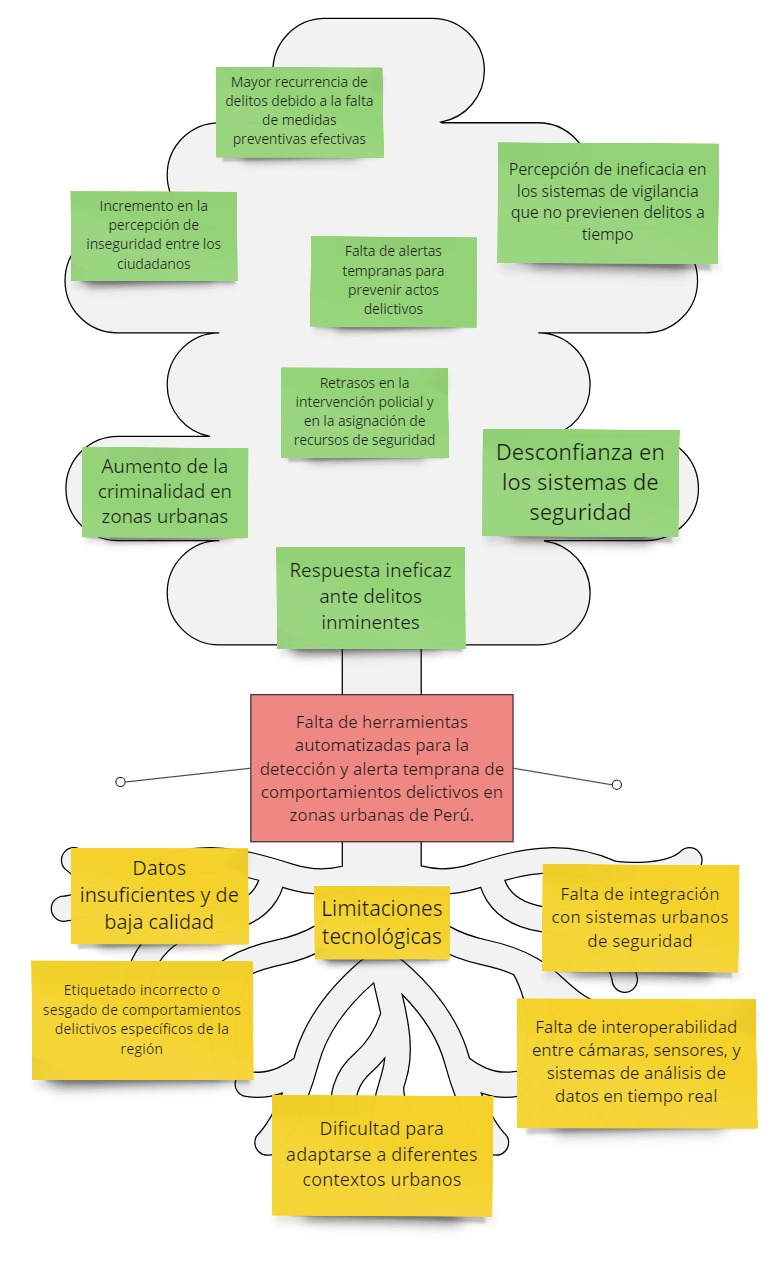
\includegraphics[width=1.00\textwidth]{anexos/Problem Tree Template (1).jpg}
			%\caption{Fuente: Elaboración propia}
		\end{center}
	\end{figure}
	\clearpage
	
	\section{Árbol de Objetivos}
	%\chapter*{Árbol de Objetivos}
	%\addcontentsline{toc}{section}{Árbol de Objetivos}
	%\renewcommand{\thechapter}{A}
	\label{anexo2}
	\begin{figure}[h]
		\begin{center}
			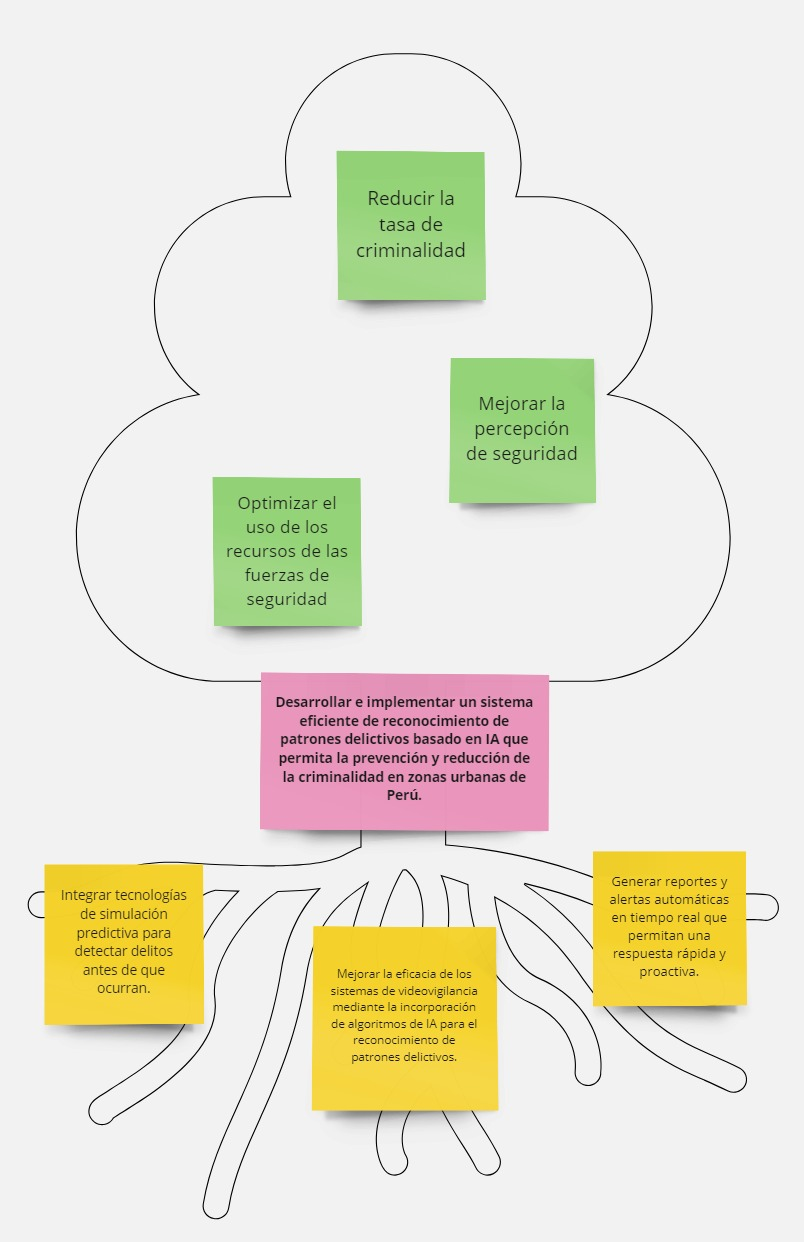
\includegraphics[width=1.00\textwidth]{anexos/arbol de objetivos (1).jpg}
			%\caption{Fuente: Elaboración propia}
		\end{center}
	\end{figure}
	\clearpage
	
	\begin{landscape}
		\section{Matriz de Consistencia}

                \begin{longtable}{| m{4cm} | m{7cm} | m{7cm} | m{7cm} |}
    \hline
    \multicolumn{4}{|c|}{\textbf{Título: Sistema predictivo de visión por computadora e IA para detección de comportamientos sospechosos y alertas tempranas en entornos urbanos}} \\ \hline
    \textbf{Aspecto} & \textbf{Problema} & \textbf{Objetivo} & \textbf{Variables} \\ \hline
    
    \textbf{Principal} & ¿Cómo puede un sistema de visión por computadora e inteligencia artificial prever y analizar comportamientos delictivos para emitir alertas tempranas y mejorar la seguridad en zonas urbanas de alto riesgo? & Desarrollar un sistema basado en IA y visión por computadora que permita detectar y predecir comportamientos delictivos en tiempo real, con el objetivo de emitir alertas tempranas para mejorar la seguridad en entornos urbanos. & \textbf{Dependiente}: Incidencia delictiva, percepción de seguridad. \newline \textbf{Independiente}: Implementación del sistema de visión por computadora e IA. \\ \hline
    
    \textbf{Específicos} & ¿Por qué no existen suficientes herramientas tecnológicas que permitan detectar comportamientos delictivos en tiempo real? & Diseñar algoritmos de visión por computadora para la identificación de posturas y elementos de disfraz como gorras o capuchas. & \textbf{Dependiente}: Eficacia en la identificación de comportamientos sospechosos. \newline \textbf{Independiente}: Uso de algoritmos de visión por computadora y detección de elementos de disfraz. \\ \hline
    
    & ¿Qué dificultades existen en el uso de simulaciones predictivas para predecir comportamientos delictivos? & Implementar un modelo predictivo que analice patrones de comportamiento sospechoso y determine la probabilidad de que ocurra un delito. & \textbf{Dependiente}: Precisión del modelo predictivo. \newline \textbf{Independiente}: Simulaciones predictivas y datos históricos de delitos. \\ \hline
    
    & ¿Cómo se pueden mejorar los sistemas de videovigilancia mediante algoritmos de IA? & Validar el sistema mediante pruebas en escenarios simulados y analizar su precisión en la emisión de alertas tempranas. & \textbf{Dependiente}: Capacidad de respuesta de las alertas. \newline \textbf{Independiente}: Algoritmos de IA y condiciones de prueba. \\ \hline
\end{longtable}
\end{landscape}

\section{Bibliografia}

\begin{itemize}
    \item Sun, T., Zhao, R., Tang, X., \& Xu, W. (2021). \textbf{\textit{Suspicious Human Activity Recognition From Surveillance Videos Using Deep Learning}}. \textit{Sensors and Actuators A: Physical}, \textbf{323}, 112633.

    \item Sultani, W., Chen, C., \& Shah, M. (2018). \textbf{\textit{Real-World Anomaly Detection in Surveillance Videos}}. In \textit{Proceedings of the IEEE Conference on Computer Vision and Pattern Recognition (CVPR)} (pp. 6479--6488).

    \item Zin, T., Win, Z., \& Myo, T. (2014). \textbf{\textit{An Integrated Framework for Detecting Suspicious Behaviors in Video Surveillance}}. \textit{International Journal of Advanced Computer Science and Applications}, \textbf{5}(2), 85--91.

    \item Redmon, J., Divvala, S., Girshick, R., \& Farhadi, A. (2016). \textbf{\textit{You Only Look Once: Unified, Real-Time Object Detection}}. In \textit{Proceedings of the IEEE Conference on Computer Vision and Pattern Recognition (CVPR)} (pp. 779--788).

    \item Chen, J., Wu, H., \& Yang, J. (2022). \textbf{\textit{Anomaly Detection Using Edge Computing in Video Surveillance}}. \textit{Journal of Visual Communication and Image Representation}, \textbf{87}, 103564.

    \item Hochreiter, S., \& Schmidhuber, J. (1997). \textbf{\textit{Long Short-Term Memory}}. \textit{Neural Computation}, \textbf{9}(8), 1735--1780.

    \item Gonzalez, R. C., \& Woods, R. E. (2018). \textbf{\textit{Digital Image Processing}} (4th ed.). Pearson Education.

    \item Krizhevsky, A., Sutskever, I., \& Hinton, G. E. (2012). \textbf{\textit{ImageNet Classification with Deep Convolutional Neural Networks}}. In \textit{Advances in Neural Information Processing Systems}, \textbf{25}, 1097--1105.

    \item Shi, W., Cao, J., Zhang, Q., Li, Y., \& Xu, L. (2016). \textbf{\textit{Edge Computing: Vision and Challenges}}. \textit{IEEE Internet of Things Journal}, \textbf{3}(5), 637--646.

    \item Dietterich, T. G., Lathrop, R. H., \& Lozano-Pérez, T. (1997). \textbf{\textit{Solving the Multiple Instance Problem with Axis-Parallel Rectangles}}. \textit{Artificial Intelligence}, \textbf{89}(1--2), 31--71.

    \item Cho, K., Merrienboer, B. V., Bahdanau, D., \& Bengio, Y. (2014). \textbf{\textit{On the Properties of Neural Machine Translation: Encoder-Decoder Approaches}}. \textit{arXiv Preprint}.

    \item Marras, C., Canning, C. G., \& Goldman, S. M. (2020). \textbf{\textit{Parkinson’s Disease Across Races and Ethnicities: A Global View}}. \textit{Movement Disorders}, \textbf{35}(10), 1747--1757.
\end{itemize}